\documentclass[10pt]{book}

\usepackage{todonotes}

\graphicspath{{res/img/}}

\author{Polonio Davide}
\title{A thesis draft}
% The outline'd be something like this:
%  Thesis outline
% 
% - Introduction about the VIBES project (context, 5G, the need for a new 
% network architecture, proposed solution, requisites)
%   + Related works
% - Analysis of the available technologies (kubernetes, openstack, openvswitch, 
% Docker, Docker swarm)
%   + Choseen tecnhologies and description of the 'reason why'
% - Project description
%   + Initial solution with Openstack and Tacker
%   + From Tacker to Openbaton
%   + From Openbaton with Openstack to Openbaton with Docker
%   + Exploration of Docker orchestrators (Swam vs Kubernetes)
%   + Kubernetes internal composition (GlusterFS, Ingress, Harbor, metrics)
%   + Openbaton and Kubernetes integration (lack of a implemented Driver, 
% integration with existinf VNFM)
% - Case study
%   + Analysis of TCP/UDP performance
% - Results
% - Future works
% - Conclusions

\makeindex
\begin{document}
 \maketitle
 

 % This is just a draft, nothing suitable for the final product: sources are in 
 % form of a footnote
 
 % --- INTRODUCTION ---
\chapter{Introduction}
\label{chap:intro}

 Through the history of internet, many factor changed and new innovations came,
but at the end of the day a foundamental key remained: TCP/IP performance are, 
indeed, what the users unconsciously want.\todo{Idea: talk about how TCP/IP 
performes quite well in wired connections, while in wireless one, such as 
wireless/satellite, sucks ass} In this context network optimization plays an 
important role, and it is for this reason that network packets are processed 
while traversing the network in order to make their transmission as fast as 
possible. On top of that, mobile traffic is continuously surging every year, 
with the backbones having more and more data to process. In this context, 
in-hardware VNF solutions are becoming less efficent. Their time-to-deploy, in 
fact, is very high compared to the requirements of the network. With this 
trend, in-hardware solutions will not be able to keep up. Is with this 
considerations that software solutions are being proposed to become the new way 
to deploy network components. While less efficent, they are faster to bring them 
up, offering an unprecedented flexibility\footnote{SDN/NFV-Based Mobile Packet 
Core Network Architectures: A Survey}. Furthermore, new virtualization 
technologies such as Cloud computing and Docker are becoming more and more 
mature for being employed in large-scale production environments, where new 
frameworks, called orchestrators (e.g. Kubernetes, Docker Swarm), allow to 
easily manage the application lifecyle, i.e. deployment, scale up/down
and finally, removal.

\section{The VIBES project}
 
 This thesis is part of the VIBES project\todo{Talk about VIBES project, add
some reference, explain what it is.}, where the necessity for better TCP/IP
transmission through satellite connections is the main requirement. To
reach this goal, the project specifications suggest to exploit the 5G incoming
technology and use the NFV-MANO architecture to perform first packets
elaboration and performance improvment and finally TCP/IP satellite chunk
optimization with the Performance Enhancing Proxy (PEP). The VIBES project
proposed five technical requirements:
\begin{enumerate}
 \item Analysis of the applicability of current and new Internet protocols in
the proposed VNF-PEP architecture
 \item Implementation of a VNF-PEP prototype
 \item Building of a PoC test platform
 \item VNF-PEP validation and performance tests on 5G use-cases
 \item Demonstration testbed management
\end{enumerate}

\subsection{VNF-PEP architecture and internet protocols}

The analysis of this topic revealed to be trivial: since internet has many
different protocols that would become infeasible to support all of them at the
same time, packet incapsulation present itself as the only faseable solution:
every packet incoming in the VNFs has already been incapsulated by the MANO,
\todo{Not sure about this, please give it a check - Not sure but I think that
it is not part of the MANO the encapsulation of the packets. Also I think that
the main purpose of UDP encapsulation is not to hide the protocol used on the
edges but 1) usa a ``quick protocol to exchange data among VNFs and 2) we are
hiding the path not the protocol itself. As we were discussing, we are creating
some sort of proxy, so the aim will be the same even if we support a plethora
of protocols.''} making the whole architecture indipendent from the protocol a
particolar flux of data uses. To achieve this, TUN/TAP
\todo{Find out acronym - EPKT? (Encapsulated PacKeT)}
interfaces were used to deploy a tunnel between VNFs, allowing them to pass
packets encapsulated in UDP ones.

\subsection{VNF-PEP prototype}

Since our goal shifted into creating a MANO testbed, our prototype doesn't
include PEP. The VNF architecture was shaped following the container
orchestrator we decided to use: Kubernetes.

\subsubsection{About Kubernetes}

As already introduced before, Kubernetes is an open source software framework
specialized in container management and orchestration. Developed by Google in
??\todo{Find out the actual date} and written in Go, it allows different
machines (called nodes from now on) to create an abstraction layer and to form
a cluster where is possible to run Docker containers without brothering about
hardware constraints. Nodes can have specific roles and specialization, all of
them managed by one or many master nodes, that actually manage the
orchestration.
On top of that, Kubernetes is virtualization-agnostic, meaning that it offers
the possibility to change the virtualization software in use (i.e. from
Container-based technology to Virtual machine software).
\begin{figure}[h]
 \centering
 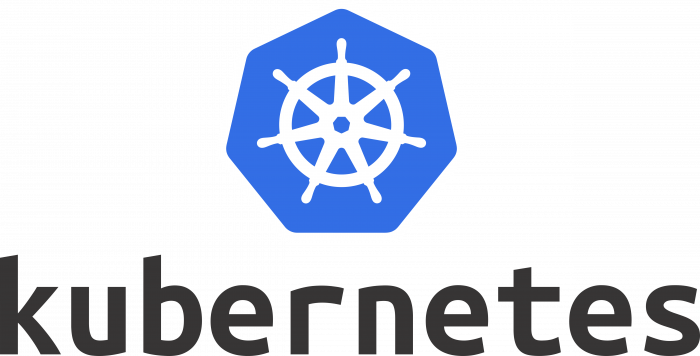
\includegraphics[scale=0.35]{kubernetes_logo}
 \caption{Kubernetes Logo}
 \label{chap:intro:img:k8s_logo}
\end{figure}


\subsubsection{About Docker}

In recent years, with the new hardware capabilities and the recent development
of in-kernel virtualization systems (such as Hyper-V) this technology
begin to be adopted. Virtualization allows to run different systems on the
same machine, making them completely isolated and then more resilient to
failures. The back of the medal, though, is that virtual machines require large
amount of resources, especially memory, because solutions like copy-and-write
of in-memory pages are not viable anymore (since the kernel gets duplicated
too), leading to duplication of loaded libraries and assets in the memory of
the host.
For large deployment containing only simple services (e.g. a backend
application serving a website or a database) this ends up in a waste of
resources. \todo{Talk about lxc containers and how Docker solved magically the
problem.} It's here that, in ??\todo{Find Docker date of birth}, Docker was
created, basing its solution on an already existing product: Linux Container
(LXC). From this framework, Docker built an entire ecosystem, consisting in a
client/server model giving the possibility for users to simply launch, scale and
delete containers (locally or remotely with Docker-machine), a repository
system where images, a layer-based ``core'' where containers start running from
when they are launched, can be stored and tagged in a sort of version control
system. Finally, another couple of solutions, called Docker-compose, and Docker
Swarm have the purpose to, respectively, orchestrate containers in a single or
a clustered system.
\begin{figure}[t]
 \centering
 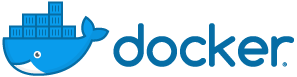
\includegraphics[scale=0.7]{docker_logo}
 \caption{Official Docker logo}
 \label{chap:intro:img:docker_logo}
\end{figure}


\paragraph{Docker Swarm} Introduced in ??\todo{Find Docker Swarm date of
birth}, Docker Swarm allows multiple Docker nodes to cluster together and be
seen as one logical unit. This layer completely makes the underlying
infrastructure transparent: data management, as network one, are totaly managed
by Docker. Recently, Docker-compose support has been introduced, making
this one-node tool available for clustered systems. At the end of the day, on
one hand Docker Swarm provides an easy way to set up a cluster system with all
the tools configured out-of-the-box, without the necessity to set networking
configurations or installing ad-hoc storage solutions. On the other hand,
though, it doesn't have all the personalization options that Kuberentes offers,
thus making the product less flexible. This foundamental characteristic,
although, makes the two solutions have different use cases leading to different
market needs. \todo{Add Docker Swarm}

\paragraph{Docker-compose} As briefly discussed above, Docker-compose is a tool
that allows services orchestration. It automates most of the tasks that should
be performed by hand when launching one or multiple docker containers. It's
particulary useful when more continers have to interact together,
because\todo{Write down docker-commpose functionalities and describe the product
a little bit} all the services rules are described in a simple YAML file.
With the birth of Docker Swarm, work has started to port this tool to the Swarm
framework. At the time of this writing, the procedure to port a Docker-compose
configuration in Docker Swarm is still not completely transparent, and it
requires a sort of compilation, where Docker-compose bundles all the
necessaries resources into a binary file that Docker Swarm will use to allocate
the necessary resources.

\vspace{0.5cm}

Starting with the first step of creating a MANO able to process incoming data
packets through VNF functions, we encountered that many networking tools
already present in the market required some tweaking and some integrations,
shifting our goal to create a complete  European Telecommunications Standards
Institutes (ETSI) Management and orchestrator (MANO) testbed instead, following
the specifications suggested in the RFC 7665, thus implementing only the first
three requisites, without digging in the satellite data flow optimization. In 
particular, we discovered how, these tools, were suitable to create ETSI MANO 
and VNFs using virtual machine or exploiting cloud tecnhologies, while they 
were not designed with enough flexibility to integrate with Docker. In the next 
chapter we are going to take a deep analysis of the cited technologies, in 
order to provide to the reader enough context to be able to understand our 
design choices we are going to describe later.


\noindent With this in mind, we performed a requirements analysis described in 
the next chapter.\todo{This should be put at the end of the introduction.}

\chapter{Project Analysis}
\label{chap:prjan}

As in chapter~\ref{chap:intro}, the creation of a full ETSI MANO compliant
architecture, following the suggestions described in RFC 7665, require the
integration of multiple tools (some of them have been already briefly introduced
in~\ref{chap:intro}). The tools were choosen after their analysis, where pro and
cons have been studied and compared to the necessity of this thesis. Since the
project has been developed with the cloud provided by the University of Padua,
Openstack (which a product analysis can be found later
in~\ref{chap:prjan:sec:openstack}) has been used as base for our deployments.

\section{Architecture overview}

During the testbed development the software architecture diverged from the 
original one, experiencing different evolutions and modifications.

\subsection{VIBES architectural description}

In the original VIBES architectural design, based on leveraging virtualization 
technologies, is possible to identify different macro-components, each of these 
specialized in fullfilling a specific goal. For the ETSI standards, the Network 
Function Virtualization (NFV) design should be composed as follows:
\begin{figure}[t]
 \centering
 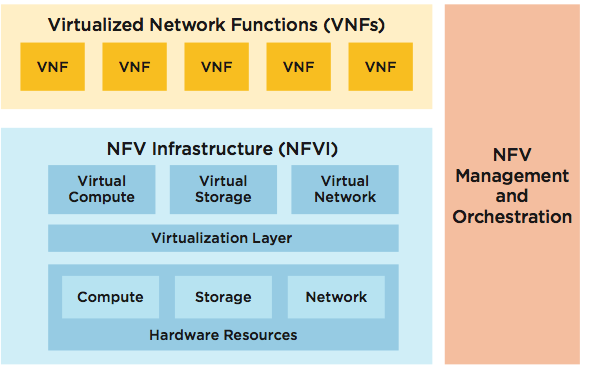
\includegraphics[scale=2]{etsi_arch}
 \caption{A schematic image representing the high level NFV architecture 
proposed by ESA.}
 \label{chap:prjan:img:etsi_arch}
\end{figure}

\begin{itemize}
 \item Network Function Virtualization Infrastructure (NFVI): it's the heart of 
the whole computation component, and here three sub-domains can be identified:
\todo{Expand this section}
\begin{itemize} 
 \item \textbf{Hypervisor domain} that is composed of the Virtual Compute, the 
Virtual Storage, and the Virtualization Layer. These components are used to 
virtualize the computational and storage resources, providing a layer for 
accessing it.
 \item \textbf{Compute domain} composed by the Physical Compute and the 
Physical Storage. These are the real resources which are virtualized via 
software.
 \item \textbf{Infrastructure domain} which has the Physical Network, and its 
virtualized counterpart as made available by the Virtualization Layer.
\end{itemize}

In conventional virtualization systems these resources are usually separated
from the host operating system, providing better isolation but wrost
performance. The ETSI infrastructure, instead, tries with container
virtualization technology to push for a better NFV responsiveness\todo{Check
  term - I don't think it actually exists}, removing the additional operating
system (called ``guest'' OS) required by the usual hypervisor-oriented approach.

To realize the required components, specific tools were suggested in the VNF 
technical proposal: regarding the NFV (network infrastructure) domain 
Docker-Compose was proposed as a viable solution, while to store PEP instances 
docker swarm was described as a possible candidate.

We performed an accured analysis of the tools choosen based on their maturity, 
on the community and on the technical support offered (e.g. user manuals, 
developer documentation), which, at the end, commited us to choose different 
tools from the suggested ones. A detailed description of the architectural 
implementation can be found in chapter~\ref{chap:archimpl}.

\end{itemize}


\section{SFC packet transmission strategies}

As today, when a packets gets send from a seder $S$, to a receiver $R$, the 
packet gets travelling to te backbone receive appropriate in-hardware packet 
processing before being received by $R$. During this elaboration, it is 
important to maintain the transparency of the connection, so that the network 
users are not aware of the packets elaboration at all. To perform that, many 
solutions are available: TUN/TAP packet incapsulation, IP Encapsulation within 
IP or TCP session recreation (know also as TCP split).

TUN/TAP and IP Encapsulation within IP (initially defined in RFC 2003 with the 
aim to deliver IP packets over Mobile IP for mobile networks) maintain the 
connection transparency incapsulating the packet in another one.
\begin{figure}[t]
  \centering
  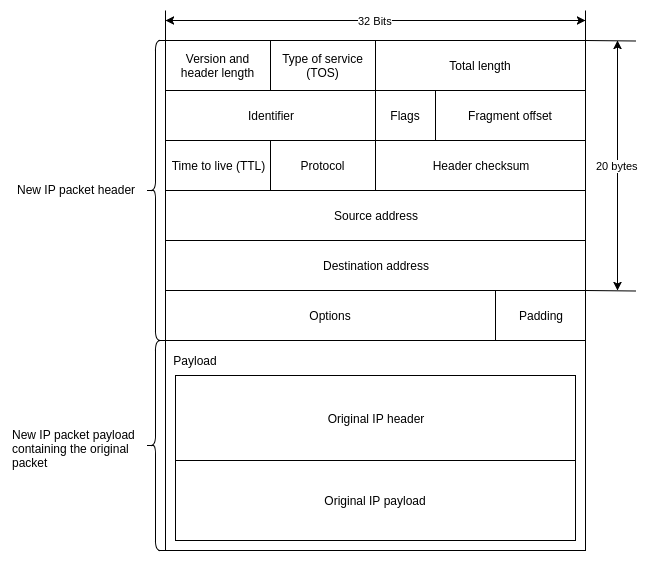
\includegraphics[scale=0.5]{IPoverIP}
  \caption[IP Encapsulation within IP packet schema]{A schema of IP 
Encapsulation within IP. Is noticeable how the original packet becomes the 
payload of a new one, thus being encapsulated. All the informations regarding 
the original packet remains untouched: when this kind of packet gets send 
from a machine to another, the OS will remove the new packet header and will 
present to the user-space program receiving the data its payload: a IP 
packet. Packets encapsulation can be applied with higher layers too, thus 
allowing for TCP and UDP packet incapsulation.}
  \label{chap:prjan:img:ip_over_ip}
\end{figure}


In this way, the original packet remains preserved and it becomes the new packet
payload, that can be elaborated and modified accordingly, until it gets 
decapsulated and sent to $R$ eventually. When $R$ receives the packet, it is 
not be aware of the packet elaboration, since all the original headers were 
preserved (or slightly modified). In particular, IP Encapsulation within IP 
allow the packets to make intermediate destinations that otherwise would not be 
selected.
TCP session recreation, instead, ``split'' the TCP session in two endpoints: an 
Ingress, that manage the connection with the client and an Egress, that 
communicate with the packet receiver creating a multi-overlay-hop path where 
for each hop there is an possible indipendent TCP connection. In order to 
achieve that, a session table needs to be established and continuously updated, 
while TCP headers need to be accordingly modified to allow data transmission 
through the Ingress and Egress points. Nonetheless, care should be given to 
packets path: in order to avoid ill-calculated congestion windows, the incoming 
packets need to follow the same (or an equivalent one) path for the same 
instatiated connection. This phenomenom is based on the intermediate proxies 
that create the route: it is the case, for example, when an intermediate node 
sends back a spoofed ACK before the original packet is delivered to the real 
consegnee. In this senario, the sender, unaware of the proxy, will miscalculate 
the sending window based on the too low RTT.
Other problems of TCP splitting are reliability and security, especially because
the end to end TCP logic is no longer maintained: a server failure may cause to
an unaware client to believe that all the packets have reached the destination.
TCP session recreation seems burdersome and it doesn't seem to add any
significant benefit at the first sight, but it offers the flexibility to perform
extensive packet manipulation: since the packet its recreated every time at the
Ingress and Egress points, while in the Network Function Virtualization
Infrastructure (NFVI), the original packet can be stripped of its headers (that
could be saved in the session table) to slightly improve internal packet
transmission. \todo{Insert TCP session recreation schema} On top of that, it
offers the possibility to use different TCP flavours, hence increasing the
communication speed in heterogeneous networks (e.g. in case of satellite
connections TCP Hybla can be employed, while it is known that HighSpeed TCP
gives best results when applied in optical fiber-based connections).

During the testbed development we first tried the TUN/TAP solution, that 
revealed to be not completely transparent and with major performance drawbacks 
(i.e. packet transmission in a LAN connection reached latencies of 50ms) 
\todo{Explain the constraint of point-to-point connections, while we need 
dynamic SFC)}, so we choose to opt for a TCP session recreation solution, 
implementing a little back-end with the aim of saving in a persistent storage 
the SFC the packet has to perform and additional metadata.

\todo{Explain TCP session recreation}

\section{Openstack}
\label{chap:prjan:sec:openstack}
Created in ??\todo{Find out Openstack date of creation}, 
Openstack allows on-permise cloud installations, using bare-metal resources to 
provide common cloud services as object storage, virtual machine deploy, 
virtual networking. Furthermore its modularity offers the possibility to add 
additional components, even proprietary, to achieve a complete cloud solution.
\begin{figure}[t]
 \centering
 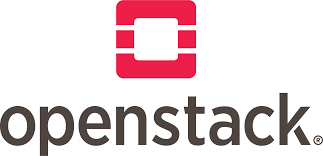
\includegraphics[scale=0.58]{openstack_logo}
 \caption{Openstack logo}
 \label{chap:prjan:img:openstack_logo}
\end{figure}



\todo{This section needs to be expanded a lot!!! In particular, we should put 
some focus about VNF and MANO, introducing them}





\subsubsection{Other technologies}\todo{Talk somehow of the other tecnhologies}
\paragraph{Openvswitch}
\paragraph{Openbaton} Created by the Institute Fraunhofer, it's a open-source, 
customizable NFV MANO-compliant framework, that offers many configurations 
options, and since it's written in Java, there is the possibility to add 
components (plug-ins) dynamically. Openbaton can be installed as a normal 
computer program (they offer packages for the most common distros) but it can 
be deployed on Docker containers too. It's designed to work with cloud 
providers like Amazon or Google Compute engine, but it offers compability with 
on-permise cloud solutions like Openstack, where it deploys virtual machines 
using the API the platform offers. It can store VNF configurations saved as 
TOSCA YAML\todo{What does TOSCA mean? Find out} and it can handle multiple 
PoPs\todo{Write down PoP meaning}. It offers a VNF lifecyle management 
out-of-the-box, with the possibility to customize it based on the user needs. 
Its modular design allows developers to change parts of the codebase with 
custom ones, making the product really flexible to different platforms. 
Performing this operation requires a deep knowlege of the framework though.
\begin{figure}[h]
 \centering
 
\includegraphics[scale=0.45]{openbaton_logo}
 \caption{Openbaton logo}
 \label{chap:prjan:img:openbaton_logo}
\end{figure}

\paragraph{SDN?}

\chapter{Architectural implementation}
\label{chap:archimpl}
\end{document}
